\chapter{Results}\label{cha:results}

This section will present and discuss the results from our experiments.
The modified SSD model presented in Section~\ref{sec:method-arch} is trained according to the training procedure given in Section~\ref{sec:method-exp-setup}.
Section~\ref{sec:results-baseline} presents the performance of the baseline model. 
The results from experiments pertaining to RQ1 and RQ2 are presented in Section~\ref{sec:results-simplification} and Section~\ref{sec:results-sharpness} respectively.
Unless specified otherwise, all performance metrics given in this section are measured on the test split of the dataset.
For measuring mAP we use an IoU of 0.5 as the acceptance threshold, and follow the interpolation method specified in Equation~\ref{eq:average-precision}

\section{Baseline model}\label{sec:results-baseline}
\begin{figure}[htbp]
    \centering
    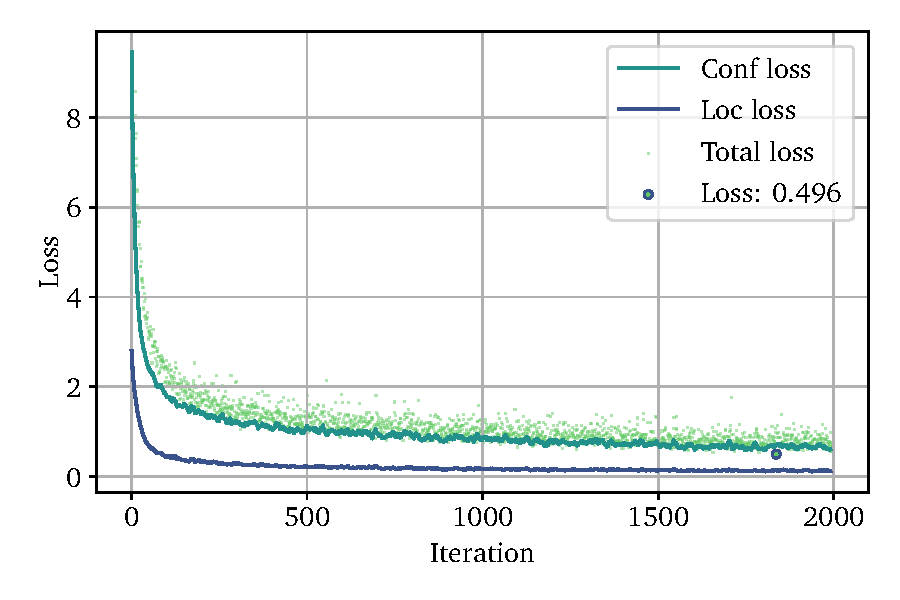
\includegraphics[width=0.7\textwidth]{figs/results/baseline/loss2.pdf}
    \caption[Baseline training procedure]{%
Training procedure for the baseline model over 2000 iterations.
The iterations are given on the horizontal axis are represent one forward-backpropagation run with one mini-batch, while the mini-batch averaged loss is given in the vertical axis.
The raw total loss values are shown with semi-transparent green points.
The solid lines show the moving means for the two individual loss components.
The green line shows the confidence loss component, while the blue line shows the localization loss component.
The mini-batch with the lowest total loss is annotated with a green circle and occurs after the 1800th iteration with a loss of 0.496.
    }\label{fig:method-baseline-loss}
  \end{figure}

We start by presenting the results from training the model in its baseline configuration. 
The training procedure is given in Figure~\ref{fig:method-baseline-loss}.
The stochastic variation in the loss curve is characteristic for mini-batch training. 
We can also see that the confidence loss accounts for most of the total loss throughout the training process.
The components of the loss function (Equation~\ref{eq:loss}) are independent, meaning that their ratio does not indicate a difference in performance at the two different tasks.
We do however observe that the model performs better at localization than classification.
Logically this follows from the realization that the pollen grains are all distinct from the background, but are all quite similar.
The model is therefore able to discriminate between background and pollen with relative ease, but has a harder time classifying species.

\begin{figure}[htbp]
    \centering
    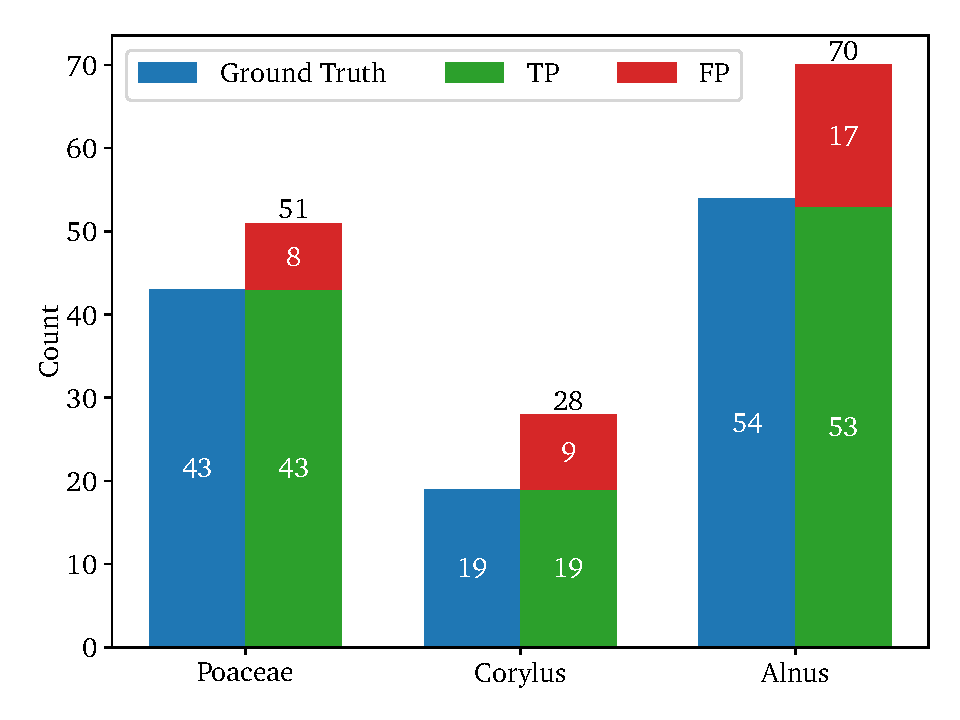
\includegraphics[width=0.7\textwidth]{figs/results/baseline/detections_test.pdf}
    \caption[Detections by type by class for the baseline on the test split] and an \(F_1\) score of \textbf{86.8\%}.
Looking at predictions overall the recall is very high at 99.1\%, while precision is quite a bit lower at 77.2\%.
Figure~\ref{fig:results-baseline-detections} breaks down all the detections made, the main observation is that false positive predictions are the almost singular source of error.
37\% of false positives are miss-localizations, i.e.~an unlabeled entity is identified as a pollen grain.
These entities are either non-pollen particles or pollen grains from unlabeled species.
The remaining 63\% of false positives are miss-classifications, i.e.~the bounding box does correspond to a ground truth, but the class is incorrect.

\begin{figure}[htbp]
  \centering
  \begin{subfigure}[t]{0.4\textwidth}
    \centering
    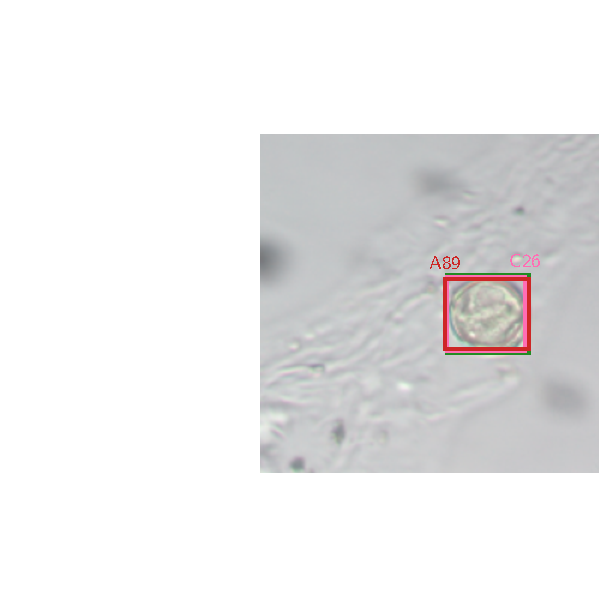
\includegraphics[width=\textwidth]{figs/results/baseline/Snap-408.pdf}
  \end{subfigure}%
  \hspace*{0.04\textwidth}
  \begin{subfigure}[t]{0.4\textwidth}
    \centering
    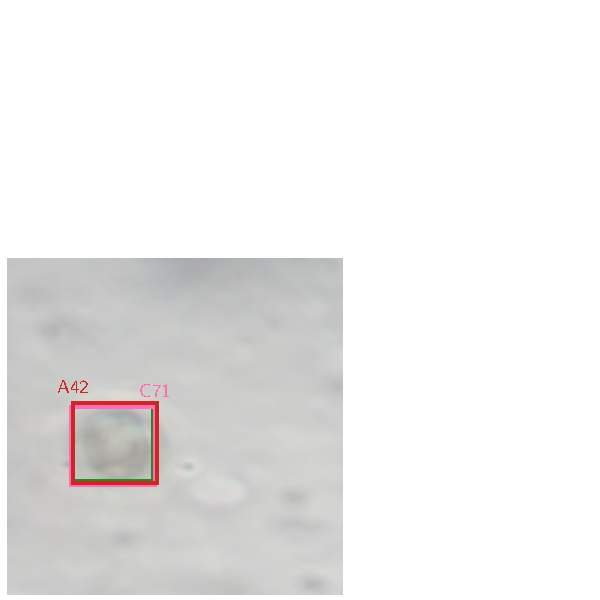
\includegraphics[width=\textwidth]{figs/results/baseline/Snap-028.pdf}
  \end{subfigure}
  \caption[Predictions showing TP overlapped by FP from different class]{Two predictions with GT in \textcolor{nicegreen}{green}, TP in \textcolor{red}{red}, and FP in \textcolor{nicepink}{pink}.
The labels give the first letter of the class and the prediction confidence in the range [0,100].
All TP labels are placed at the NW corner of the bounding box.
The FP labels are placed at the other three corners according to class.
In the left image, a FP box is predicted with a lower confidence than the TP\@.
In the right image, the FP corylus prediction has a higher confidence than the TP alnus prediction.}\label{fig:results-overlapping-predictions}
\end{figure}

Figure~\ref{fig:results-overlapping-predictions} shows two test samples containing overlapping true and false positive predictions.
This is due to the NMS filtering algorithm being run for each class independently, which causes double predictions in cases where predictions for multiple classes are produced for the same pollen grain.

A remedy for this was implemented and tested where NMS was applied to all detections after the initial per-class NMS\@.
The results from this were ambiguous; The precision did improve due to the decreased number of FP predictions, but the decrease in TP predictions caused a similar decrease in recall.
In Figure~\ref{fig:results-overlapping-predictions} (right) for example, the correct prediction would get filtered out.
We maintain that with an improved classification error, this technique would be of benefit, as it would improve overall precision without sacrificing recall.

\section{Model simplification}\label{sec:results-simplification}
The first two experiments aim to explore ways in which we can reduce the computational complexity of the model without sacrificing performance.
In the first experiment we have changed the feature extraction network with light weight alternatives.
In the second we have reduced the amount of default boxes by deactivating source feature maps.

\subsection{Feature extractor}
Table~\ref{tab:result-base-network} gives the results from training the network with different feature extraction networks.
As with the baseline, all the networks are pertained on image classification datasets.
Larger networks, such as the deeper ResNet versions, could not be tested due to the memory limitations of the GPU\@.
We see a clear decrease in performance when using smaller networks, and observe monotonically decreasing values for all performance metrics.

Interestingly, the recall remains almost unchanged, meaning that the model's ability to localize pollen grains is largely maintained.
The error is in the form of noise being added on top of the correct predictions.
The performance degradation is therefore mostly due to increased classification error, creating redundant, poor predictions.
A possible explanation for this is that localization, in terms of feature engineering requirements, only requires the model to learn simple features relating to the general shape and color of a pollen grain, while classification involves more complex features that the smaller networks are not able to capture.

\begin{table}\centering
  \ra{1.3}
\caption[Performance by feature extraction network]{Summary of experimental results from testing various small feature extraction networks.
The localization score refers to the share of detection that correctly localize a GT, regardless of class.
For each network, the number of trainable parameters for both the feature extractor and whole model is given.}%
\label{tab:result-base-network}
\begin{tabular}{@{}lcrrrrcrr@{}}\toprule
  Network & \phantom{a} & \multicolumn{4}{c}{Performance} & \phantom{ab}&  \multicolumn{2}{c}{Parameters} \\
  \cmidrule{3-6} \cmidrule{8-9}
        &&  mAP &  Precision &  Recall &  Loc. &&  Extractor   & Total \\
  \midrule                                                                     
     ResNet 34 && 95.2 &      82.7  &   99.1  & 95.0  &&  \num{8.2e6} & \num{1.2e7} \\
     ResNet 18 && 92.6 &      81.9  &   97.4  & 92.8  &&  \num{2.8e6} & \num{6.7e6} \\
  MobileNet V2 && 90.4 &      67.9  &   98.3  & 86.3  &&  \num{1.3e5} & \num{9.6e5} \\  
  \bottomrule
\end{tabular}
\end{table}

\subsection{Layer activation}
In the next experiment we deactivate layers of the extra structure responsible for generating the various source feature maps.
The results are given in Table~\ref{tab:result-layer-deactivated} and do not point towards any strong trend.
The last 3 layers of the model are larger than almost all grains in the dataset, and even with cropping, it is likely that their predictions do not contribute to the loss because the default boxes they encode rarely, if ever, get matched with a ground truth.
Their inclusion then might result in parameters that do not get trained properly leading to those layers only producing noise instead of actual predictions.

For the first three layers we do observe improved mAP, but the statistical significance is questionable.
This does however call into question the importance of the larger feature maps, and strengthens our initial belief that the SSD model can be simplified without compromises to performance.


\begin{table}\centering
  \ra{1.1}
  \caption[Performance when deactivating source layers]{Summary of experimental results when deactivating various source layers.
  The source layers are ordered 1--6 with layer 1 being the most granular \(38\by38\) feature map.}%
  \label{tab:result-layer-deactivated}
\begin{tabular}{@{}llllllcrrr@{}}\toprule
  \multicolumn{6}{c}{Source layer activation} & \phantom{a} & \multicolumn{3}{c}{Performance}\\
  \cmidrule{1-6} \cmidrule{8-10}
  1 & 2 & 3 & 4 & 5 & 6 &&   mAP & Precision & Recall \\
  \midrule
  \ckm & \ckm & \ckm & \ckm & \ckm & \ckm && 95.3  & 84.6 & 99.1 \\
  \ckm & \ckm & \ckm & \ckm & \ckm &      && 95.5  & 77.4 & 99.1 \\
  \ckm & \ckm & \ckm & \ckm &      &      && 95.3  & 81.2 & 98.7 \\
  \ckm & \ckm & \ckm &      &      &      && \textbf{96.4}  & 79.3 & 99.1 \\
  \ckm & \ckm &      &      &      &      && 95.6  & 80.4 & 98.7 \\
  \ckm &      &      &      &      &      && 96.3  & 83.6 & 99.1 \\
       & \ckm &      &      &      &      && 95.7  & 85.5 & 99.1 \\
  \bottomrule
\end{tabular}
\end{table}

\section{Sharpness}\label{sec:results-sharpness}
Next we look at how sharpness of the ground truth data impacts model performance. In the first experiment we filter out the blurry images to see the effect this has on the inferences made by the model. In the second experiment we split the dataset based on sharpness and measure the models ability to make inferences across this sharpness boundary.

\subsection{Minimum training sharpness}\label{sec:results-minimum}
Our first experiment aims to explore how the sharpness of the training data effects the predictions that the model is able to make.
The results indicate that the model struggles with making inferences on grains with lower sharpness when such grains are filtered out of the training data.
Figure~\ref{fig:results-sharpness-gt} breaks down the ground truth labels into true positives and false negatives and we see that the model is failing to predict pollen grains which have a sharpness below the minimum sharpness of the training data.

Looking at the sharpness of the predictions made by the model we see a corollary trend in the false positive predictions.
In Figure~\ref{fig:results-sharpness-detections} we observe that restricting the training data creates what seems to be a threshold, bellow which the model does not make predictions.
This shows that the model is loosing the ability to even localize blurry pollen grains, becoming blind to their existence.
It seems clear that the features being learned from sharp images do not transfer to less sharp samples.

It is important to note that the sample size, especially in the case of false negatives, is quite low, which weakens arguments made based on their distributions.
What we are seeing could be described as a type of `overfitting' where the model will not generalize outside of the sharpness bound of the training data, and the implications this has for a hypothetical production system is unclear.

\begin{figure}[htbp]
  \centering
  \begin{subfigure}[t]{\textwidth}
    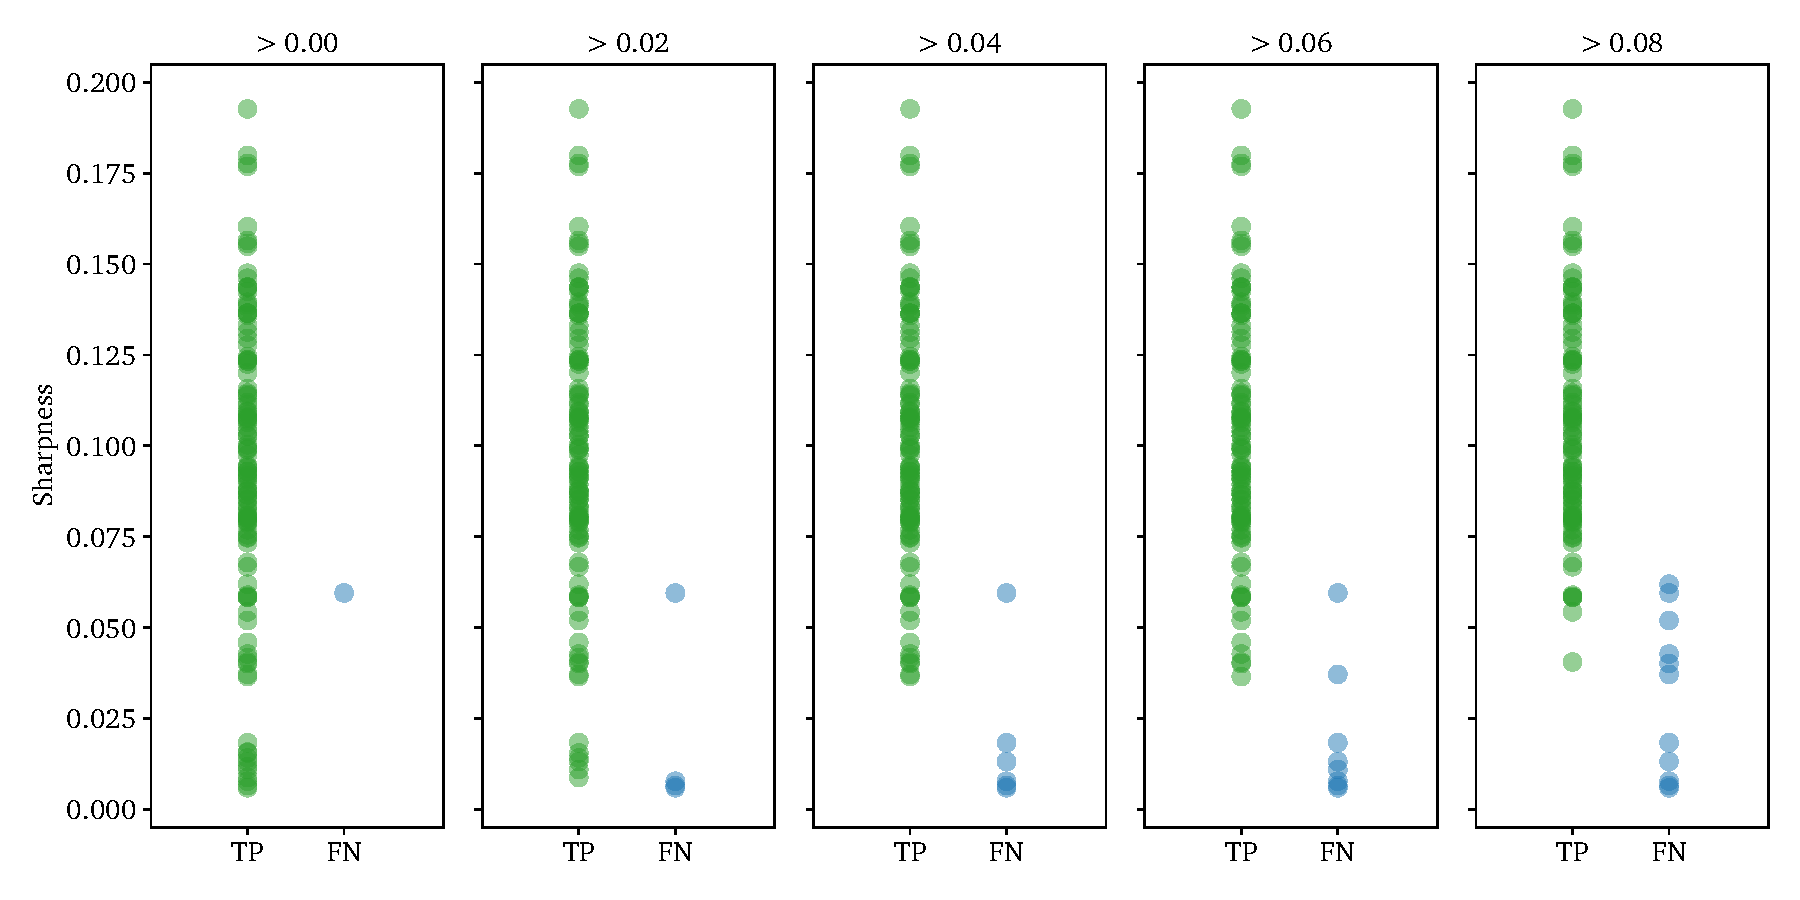
\includegraphics[width=\textwidth]{figs/results/sharpness/sharpness_TP_vs_FN.pdf}
    \subcaption{Sharpness distribution of \textit{ground truths} by prediction result in test split by minimum training sharpness}\label{fig:results-sharpness-gt}
  \end{subfigure}
  \begin{subfigure}[t]{\textwidth}
    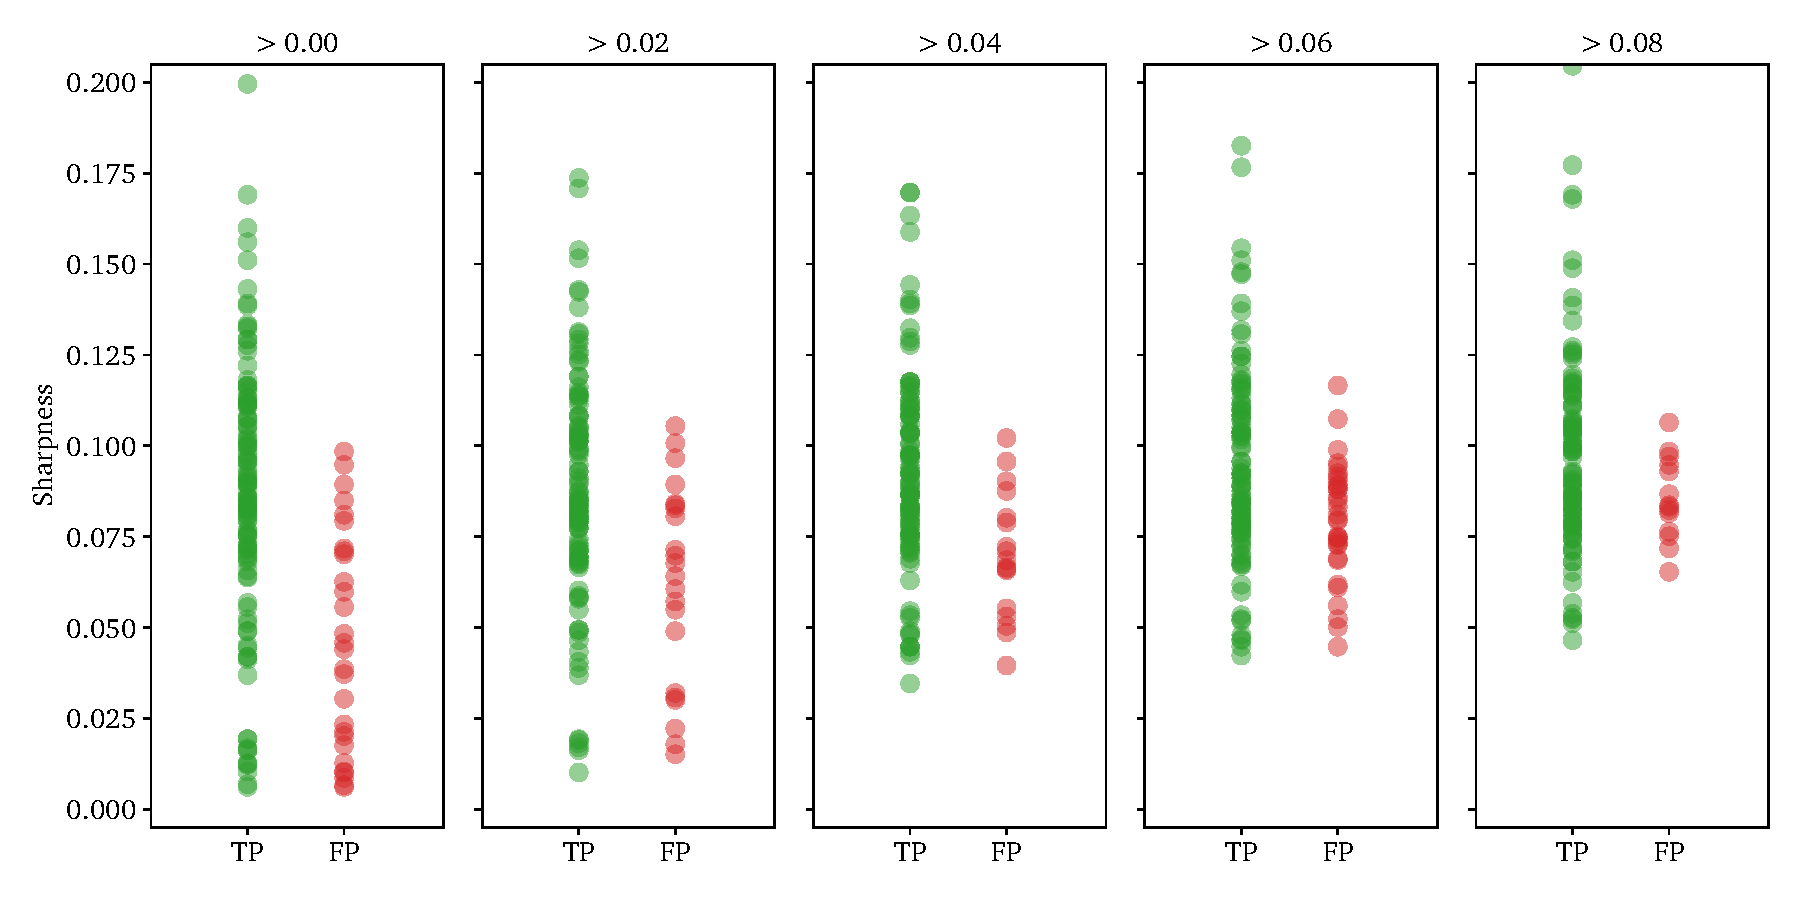
\includegraphics[width=\textwidth]{figs/results/sharpness/detection_sharpness_TP_vs_FP.pdf}
    \subcaption{Sharpness distribution of \textit{model predictions} by prediction result in test split by minimum training sharpness}\label{fig:results-sharpness-detections}
  \end{subfigure}
  \caption[Sharpness distribution of model predictions in test split by minimum training sharpness]{%
  Five experimental runs are shown, ground truth labels are filtered out of the training set by the sharpness requirement given in the plot header. In~\subref{fig:results-sharpness-gt}, sharpness is measured on original images using ground truth bounding boxes. In~\subref{fig:results-sharpness-detections}, sharpness is measured on the resampled \(300\by300\) pixel patches. This effects the scaling of the sharpness measure, and sharpness values from the two figures are therefore not directly comparable.}
\end{figure}

\subsection{Cross-sharpness inference}
For the final experiment we aim to explore how well the model is able to generalize to sharpnesses out of its training data.
The results are given as a confession matrix matching training data to testing data with the dataset being split between sharp and blurry based on the median sharpness over the entire training/testing split.
Figure~\ref{fig:results-sharpness-inference}

\begin{figure}[htbp]
  \centering
  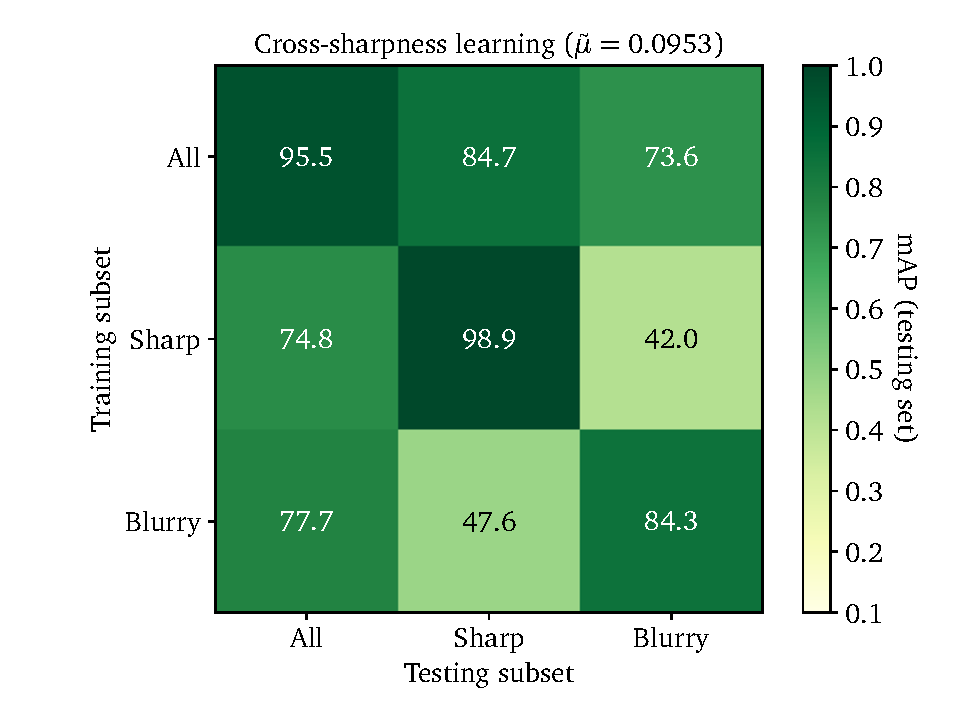
\includegraphics[width=0.9\textwidth]{figs/results/sharpness/confustion_balanced_test.pdf}
  \caption[Performance across sharpness boundary]{%

  }\label{fig:results-sharpness-inference}
\end{figure}

Our results from~\ref{sec:results-minimum} indicate poor performance at generalizing from sharp training data to blurry test data.
